\documentclass[a4paper]{article}
\usepackage{geometry}
\usepackage{graphicx}
\usepackage{natbib}
\usepackage{amsmath}
\usepackage{amssymb}
\usepackage{amsthm}
\usepackage{paralist}
\usepackage{epstopdf}
\usepackage{tabularx}
\usepackage{longtable}
\usepackage{multirow}
\usepackage{multicol}
\usepackage[hidelinks]{hyperref}
\usepackage{fancyvrb}
\usepackage{algorithm}
\usepackage{algorithmic}
\usepackage{float}
\usepackage{paralist}
\usepackage[svgname]{xcolor}
\usepackage{enumerate}
\usepackage{array}
\usepackage{times}
\usepackage{url}
\usepackage{fancyhdr}
\usepackage{comment}
\usepackage{environ}
\usepackage{times}
\usepackage{textcomp}
\usepackage{caption}
\usepackage{multirow}


\urlstyle{rm}

\setlength\parindent{0pt} % Removes all indentation from paragraphs
\theoremstyle{definition}
\newtheorem{definition}{Definition}[]
\newtheorem{conjecture}{Conjecture}[]
\newtheorem{example}{Example}[]
\newtheorem{theorem}{Theorem}[]
\newtheorem{lemma}{Lemma}
\newtheorem{proposition}{Proposition}
\newtheorem{corollary}{Corollary}


\floatname{algorithm}{Procedure}
\renewcommand{\algorithmicrequire}{\textbf{Input:}}
\renewcommand{\algorithmicensure}{\textbf{Output:}}
\newcommand{\abs}[1]{\lvert#1\rvert}
\newcommand{\norm}[1]{\lVert#1\rVert}
\newcommand{\RR}{\mathbb{R}}
\newcommand{\CC}{\mathbb{C}}
\newcommand{\Nat}{\mathbb{N}}
\newcommand{\br}[1]{\{#1\}}
\DeclareMathOperator*{\argmin}{arg\,min}
\DeclareMathOperator*{\argmax}{arg\,max}
\renewcommand{\qedsymbol}{$\blacksquare$}

\definecolor{dkgreen}{rgb}{0,0.6,0}
\definecolor{gray}{rgb}{0.5,0.5,0.5}
\definecolor{mauve}{rgb}{0.58,0,0.82}

\newcommand{\Var}{\mathrm{Var}}
\newcommand{\Cov}{\mathrm{Cov}}

\newcommand{\vc}[1]{\boldsymbol{#1}}
\newcommand{\xv}{\vc{x}}
\newcommand{\Sigmav}{\vc{\Sigma}}
\newcommand{\alphav}{\vc{\alpha}}
\newcommand{\muv}{\vc{\mu}}

\newcommand{\red}[1]{\textcolor{red}{#1}}

\def\x{\mathbf x}
\def\y{\mathbf y}
\def\w{\mathbf w}
\def\v{\mathbf v}
\def\E{\mathbb E}
\def\V{\mathbb V}

% TO SHOW SOLUTIONS, include following (else comment out):
\newenvironment{soln}{
    \leavevmode\color{blue}\ignorespaces
}{}


\hypersetup{
%    colorlinks,
    linkcolor={red!50!black},
    citecolor={blue!50!black},
    urlcolor={blue!80!black}
}

\geometry{
  top=1in,            % <-- you want to adjust this
  inner=1in,
  outer=1in,
  bottom=1in,
  headheight=3em,       % <-- and this
  headsep=2em,          % <-- and this
  footskip=3em,
}


\pagestyle{fancyplain}
\lhead{\fancyplain{}{Homework 3}}
\rhead{\fancyplain{}{CS 760 Machine Learning}}
\cfoot{\thepage}

\title{\textsc{Homework 3}} % Title

%%% NOTE:  Replace 'NAME HERE' etc., and delete any "\red{}" wrappers (so it won't show up as red)

\author{Dario Placencio\\908 284 6018}

\date{}

\begin{document}

\maketitle 


\textbf{Instructions:} 
Use this latex file as a template to develop your homework. Submit your homework on time as a single pdf file to Canvas. Late submissions may not be accepted. Please wrap your code and upload to a public GitHub repo, then attach the link below the instructions so that we can access it. You can choose any programming language (i.e. python, R, or MATLAB). Please check Piazza for updates about the homework.


\textbf{Github Repo:}
\url{https://github.com/placenciohid/ECE760-Homework/blob/a07d70fbccf8c85da945eb97a608062c0fa8b51a/Homework%203/Homework%203%20-%20Dario%20Placencio.ipynb}
	

\section{Questions (50 pts)}
\begin{enumerate}
\item (9 pts) Explain whether each scenario is a classification or regression problem. And, provide the number of data points ($n$) and the number of features ($p$).

\begin{enumerate}
	\item (3 pts) We collect a set of data on the top 500 firms in the US. For each firm we record profit, number of employees, industry and the CEO salary. We are interested in predicting CEO salary with given factors.
	
	\begin{soln}  Given we have 500 companies, we have 500 data points. These come with 4 features each: (1) Profit, (2) # of Employyees, (3) Industry, so 3 variables. Also the label/target variable of the CEO Salary is present. The problem represents a Regression, since the predictions aims for an particular amount. \end{soln}
	
	\item (3 pts) We are considering launching a new product and wish to know whether it will be a success or a failure. We collect data on 20 similar products that were previously launched. For each product we have recorded whether it was a success or failure, price charged for the product, marketing budget, competition price, and ten other variables.
	
	\begin{soln}  Here, we have 20 data points, with 13 features, and a problem that has a classification nature, since the intend is to predict is either success or failure, being a binary classification. \end{soln}
	
	\item (3 pts) We are interesting in predicting the \% change in the US dollar in relation to the weekly changes in the world stock markets. Hence we collect weekly data for all of 2012. For each week we record the \% change in the dollar, the \% change in the US market, the \% change in the British market, and the \% change in the German market.
	
	\begin{soln}  For this one, the data points are 54 (weeks in a year), the features are 4: USD, USD Market, British, German. And the problem has a regression nature, since the prediction aims towards a percentage change, looking the value itself. \end{soln}
	
\end{enumerate}

\item (6 pts) The table below provides a training data set containing six observations, three predictors, and one qualitative response variable.

\begin{center}
	\begin{tabular}{ c  c  c  c}
		\hline
		$X_{1}$ & $X_{2}$ & $X_{3}$ & $Y$ \\ \hline
		0 & 3 & 0 & Red \\
		2 & 0 & 0 & Red \\
		0 & 1 & 3 & Red \\
		0 & 1 & 2 & Green \\
		-1 & 0 & 1 & Green \\
		1 & 1 & 1 & Red  \\
		\hline
	\end{tabular}
\end{center}

Suppose we wish to use this data set to make a prediction for $Y$ when $X_{1} = X_{2} = X_{3} = 0$ using K-nearest neighbors.

\begin{enumerate}
	\item (2 pts) Compute the Euclidean distance between each observation and the test point, $X_{1} = X_{2} = X_{3}=0$.
 
	\begin{soln}  The calculated Euclidean distances from each point to the point of interest are as follows:

		$$
		\begin{array}{cccc}
		\hline
		X_{1} & X_{2} & X_{3} & \text{Distance} \\
		\hline
		0 & 3 & 0 & \sqrt{9} = 3 \\
		2 & 0 & 0 & \sqrt{4} = 2 \\
		0 & 1 & 3 & \sqrt{10} \approx 3.16 \\
		0 & 1 & 2 & \sqrt{5} \approx 2.24 \\
		-1 & 0 & 1 & \sqrt{2} \approx 1.41 \\
		1 & 1 & 1 & \sqrt{3} \approx 1.73 \\
		\hline
		\end{array}
		$$
	
	\end{soln}
 
	\item (2 pts) What is our prediction with $K=1$? Why?
	
	\begin{soln}  The prediction with K = 1 is Green because the closest observation is Green, with a distance of 1.41. \end{soln}
	
	\item (2 pts) What is our prediction with $K=3$? Why?
	
	\begin{soln}  The prediction with K = 3 would be Red, from the 3 closest observations, 2 are Red and 1 is Green. The vote would be Red, hence the prediction. The values of these distances are 1.41, 1.73, and 2.00. \end{soln}

\end{enumerate}

\item (12 pts) When the number of features $p$ is large, there tends to be a deterioration in the performance of KNN and other local approaches that perform prediction using only observations that are near the test ob- servation for which a prediction must be made. This phenomenon is known as the curse of dimensionality, and it ties into the fact that non-parametric approaches often perform poorly when $p$ is large.

\begin{enumerate}
	\item (2pts) Suppose that we have a set of observations, each with measurements on $p=1$ feature, $X$. We assume that $X$ is uniformly (evenly) distributed on [0, 1]. Associated with each observation is a response value. Suppose that we wish to predict a test observation’s response using only observations that are within 10\% of the range of $X$ closest to that test observation. For instance, in order to predict the response for a test observation with $X=0.6$, we will use observations in the range [0.55, 0.65]. On average, what fraction of the available observations will we use to make the prediction?
	
	\begin{soln}  
		X is uniformly distributed on [0,1].\\
		We will predict the response for a test observation using the range $[x - 0.05, x + 0.05]$\\
		Given X is uniformly distributed on [0,1], the probability density function (pdf) is:
		
		$$
		f(x) = \begin{cases}
		1 & \text{if } 0 \leq x \leq 1 \\
		0 & \text{otherwise}
		\end{cases}
		$$
		
		Now, calculating the probability of the range the observation within the 10% range:
		
		$$  
		\begin{align}
		P(x - 0.05 \leq X \leq x + 0.05) &= \int_{x - 0.05}^{x + 0.05} f(x) dx \\
		&= \int_{x - 0.05}^{x + 0.05} 1 dx \\
		&= x + 0.05 - (x - 0.05) \\
		&= 0.1
		\end{align}
		$$
		
		So, the probability of the range the observation within the 10 percent range is 0.1. \end{soln}
	
	
	\item (2pts) Now suppose that we have a set of observations, each with measurements on $p =2$ features, $X1$ and $X2$. We assume that predict a test observation’s response using only observations that $(X1,X2)$ are uniformly distributed on [0, 1] × [0, 1]. We wish to are within 10\% of the range of $X1$ and within 10\% of the range of $X2$ closest to that test observation. For instance, in order to predict the response for a test observation with $X1 =0.6$ and $X2 =0.35$, we will use observations in the range [0.55, 0.65] for $X1$ and in the range [0.3, 0.4] for $X2$. On average, what fraction of the available observations will we use to make the prediction?
	
	\begin{soln}  
		Both X1, X2 are uniformly distributed on [0,1].\\
		We will predict the response for a test observation using the range $[x_{1} - 0.05, x_{1} + 0.05]$ for X1 and $[x_{2} - 0.05, x_{2} + 0.05]$ for X2\\
		Given X1, X2 are uniformly distributed on [0,1], the probability density function (pdf) is:
		
		$$
		f(x_{1}, x_{2}) = \begin{cases}
		1 & \text{if } 0 \leq x_{1}, x_{2} \leq 1 \\
		0 & \text{otherwise}
		\end{cases}
		$$
		
		Now, calculating the probability of the range x1 [0.55, 0.65] and x2 [0.3, 0.4]:
		
		$$
		\begin{align}
		P(0.6 - 0.05 \leq X_{1} \leq 0.6 + 0.05, 0.35 - 0.05 \leq X_{2} \leq 0.35 + 0.05) &= \int_{0.55}^{0.65} \int_{0.3}^{0.4} f(x_{1}, x_{2}) dx_{1} dx_{2} \\
		&= \int_{0.55}^{0.65} \int_{0.3}^{0.4} 1 dx_{1} dx_{2} \\
		&= \int_{0.55}^{0.65} x_{1} \Big|_{0.3}^{0.4} dx_{2} \\
		&= \int_{0.55}^{0.65} 0.1 dx_{2} \\
		&= 0.1 \int_{0.55}^{0.65} dx_{2} \\
		&= 0.1 x_{2} \Big|_{0.55}^{0.65} \\
		&= 0.1 (0.65 - 0.55) \\
		&= 0.01
		\end{align}
		$$
		
		We will use 1 percent of the available observations to make the prediction when considering both features, with a 10 percent range. \end{soln}
	
	\item (2pts) Now suppose that we have a set of observations on $p = 100$ features. Again the observations are uniformly distributed on each feature, and again each feature ranges in value from 0 to 1. We wish to predict a test observations response using observations within the 10\% of each feature’s range that is closest to that test observation. What fraction of the available observations will we use to make the prediction?
	
	\begin{soln}  So, from the previous answer we know that:

		For p=1, we use 10 percent or 0.1 of the observations.\\
		For p=2, we use 10 percent or 0.01 of the observations.\\
		
		These values are the product of the fractions of observations used in each individual feature's dimension. This is because, given independence and uniform distribution, the fraction of observations used in a multi-dimensional space is the product of the probabilities in each dimension.\\
		
		Extending this to 100 dimensions, we get:
		
		$$
		\begin{align}
		(0.1)^{p} &= 1.0 \times 10^{-100} \\
		\end{align}
		$$
		
		So we will use $1.0 \times 10^{-100}$ of the available observations to make the prediction when considering 100 features, with a 10 percent range. \end{soln}
	
	\item (3pts) Using your answers to parts (a)–(c), argue that a drawback of KNN when p is large is that there are very few training observations “near” any given test observation.
	
	\begin{soln}  
		This is one of the challanges impose by the "curse of dimensionality", as the number of features (or dimensions) increases, so does the distance between the data points. KNN is approach that leverages on spatial proximity to make predictions, so as the distance between the data points increases, the accuracy of the predictions decreases.\\
		Even on data sets with a large number of observations, if the number of features is large, is unlikely that the data points will be close to each other, because the distance is a exponential function of the number of features. 
	\end{soln}
	
	\item (3pts) Now suppose that we wish to make a prediction for a test observation by creating a $p$-dimensional hypercube centered around the test observation that contains, on average, 10\% of the training observations. For $p =$1, 2, and 100, what is the length of each side of the hypercube? Comment what happens to the length of the sides as $\lim_{{p \to \infty}}$.
	
	\begin{soln}  In order to calculate the lenth of the hypercube on each one of the p values, let's first define the volume of the hypercube as:

		$$
		\begin{align}
		V &= L^{p} \\
		\end{align}
		$$
		
		Where L is the length of each side of the hypercube and p is the number of dimensions.
		
		We know that percentage of observations used in each individual feature's dimension is 0.1, so:
		
		$$
		\begin{align}
		L^{p} &= 0.1 \\
		L &= 0.1^{\frac{1}{p}} \\
		\end{align}
		$$
		
		Replacing the values of 1,2, and 100 for p, we get:
		
		$$
		\begin{align}
		L_{p=1} &= 0.1^{\frac{1}{1}} = 0.1 \\
		L_{p=2} &= 0.1^{\frac{1}{2}} = 0.316 \\
		L_{p=100} &= 0.1^{\frac{1}{100}} = 0.977 \\
		\end{align}
		$$
		
		This shows that as the value of features increases, so does the length of the sides of the hypercube, getting closer to 1, representing the entire range of the feature. This means that with more features, we progresively need to consider a larger range of values to make predictions, making the "neighborhood" of the KNN model larger, and therefore less accurate. \end{soln}
	
\end{enumerate}

\item (6 pts) Suppose you trained a classifier for a spam detection system. The prediction result on the test set is summarized in the following table.
\begin{center}
	\begin{tabular}{l l | l l}
		&          & \multicolumn{2}{l}{Predicted class} \\
		&          & Spam           & not Spam           \\
		\hline
		\multirow{2}{*}{Actual class} & Spam     & 8              & 2                  \\
		& not Spam & 16             & 974               
	\end{tabular}
\end{center}

Calculate
\begin{enumerate}
	\item (2 pts) Accuracy
	\begin{soln}  

		$$
		\begin{align}
		Accuracy 
		&= \frac{TP + TN}{TP + TN + FP + FN} \\
		&= \frac{8 + 974}{8 + 974 + 16 + 2} \\
		&= \frac{982}{1000} \\
		&= 0.982
		\end{align}
		$$
	
	\end{soln}
	\item (2 pts) Precision
	\begin{soln}  

		$$
		\begin{align}
		Precision &= \frac{TP}{TP + FP} \\
		&= \frac{8}{8 + 16} \\
		&= \frac{8}{24} \\
		&= 0.333
		\end{align}
		$$
	
	\end{soln}
	\item (2 pts) Recall
	\begin{soln}  

		$$
		\begin{align}
		Recall &= \frac{TP}{TP + FN} \\
		&= \frac{8}{8 + 2} \\
		&= \frac{8}{10} \\
		&= 0.8
		\end{align}
		$$
	
	\end{soln}
\end{enumerate}


\item (9pts) Again, suppose you trained a classifier for a spam filter. The prediction result on the test set is summarized in the following table. Here, "+" represents spam, and "-" means not spam.

\begin{center}
\begin{tabular}{ c  c }
\hline
Confidence positive & Correct class \\ \hline
0.95 & + \\
0.85 & + \\
0.8 & - \\
0.7 & + \\
0.55 & + \\
0.45 & - \\
0.4 & + \\
0.3 & + \\
0.2 & - \\
0.1 & - \\
\hline
\end{tabular}
\end{center}

\begin{enumerate}
	\item (6pts) Draw a ROC curve based on the above table.
	
	\begin{soln}
		 
	\begin{figure}[h]
		\centering
		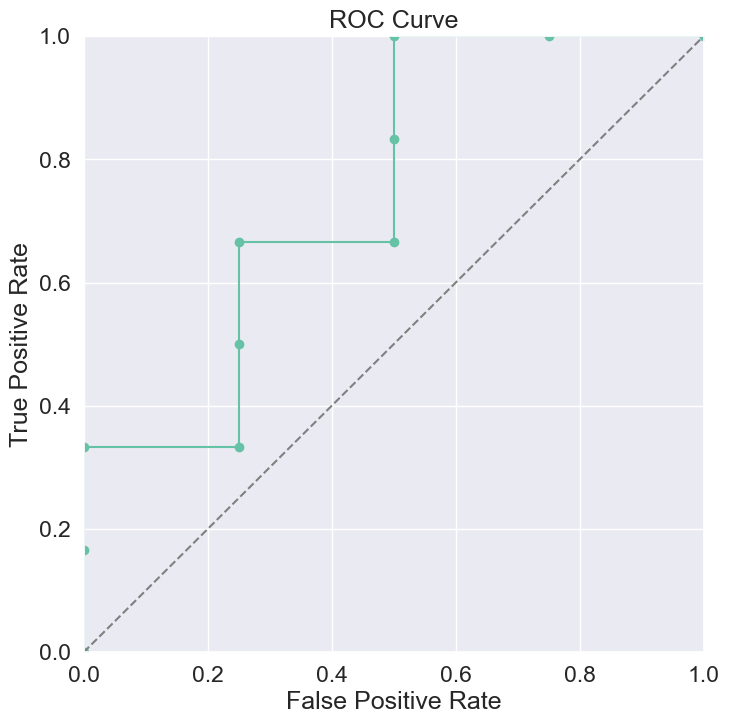
\includegraphics[width=8cm]{ROC Curve.png}
	\end{figure}
	
	\end{soln}
	
	\item (3pts) (Real-world open question) Suppose you want to choose a threshold parameter so that mails with confidence positives above the threshold can be classified as spam. Which value will you choose? Justify your answer based on the ROC curve.
	
	\begin{soln} 
		Considering the context, what I would like to avoid is to have False Positives, emails that are actually not Spam, and that I would be missing from my inbox because of missclassification.\\
		So, I would choose a threshold that would minimize the False Positive Rate (FPR), based on the values of the ROC curve, this treshold would be .85, which would give me a FPR of 0, but in comparison a little bit of a better classification of the True Positives (TPR) than the threshold of 0.95. \end{soln}
\end{enumerate}

\item (8 pts) In this problem, we will walk through a single step of the gradient descent algorithm for logistic regression. As a reminder,
$$\hat{y} = f(x, \theta)$$
$$f(x;\theta) = \sigma(\theta^\top x)$$
$$\text{Cross entropy loss } L(\hat{y}, y) = -[y \log  \hat{y} + (1-y)\log(1-\hat{y})]$$
$$\text{The single update step } \theta^{t+1} = \theta^{t} - \eta \nabla_{\theta} L(f(x;\theta), y) $$



\begin{enumerate}
	\item (4 pts) Compute the first gradient $\nabla_{\theta} L(f(x;\theta), y)$.
	
	\begin{soln}  The first gradient of the loss function is:

		$$
		\begin{align}
		\nabla_{\theta} L(f(x;\theta), y) &= \frac{\partial}{\partial \theta} L(f(x;\theta), y) \\
		&= \frac{\partial}{\partial \theta} -[y \log  \hat{y} + (1-y)\log(1-\hat{y})] \\
		&= -[y \frac{\partial}{\partial \theta} \log  \hat{y} + (1-y)\frac{\partial}{\partial \theta} \log(1-\hat{y})] \\
		&= -[y \frac{\partial}{\partial \theta} \log  \sigma(\theta^\top x) + (1-y)\frac{\partial}{\partial \theta} \log(1-\sigma(\theta^\top x))] \\
		&= -[y \frac{1}{\sigma(\theta^\top x)} \frac{\partial}{\partial \theta} \sigma(\theta^\top x) + (1-y)\frac{1}{1-\sigma(\theta^\top x)}\frac{\partial}{\partial \theta} \log(1-\sigma(\theta^\top x))] \\
		&= -[y \frac{1}{\sigma(\theta^\top x)} \sigma(\theta^\top x) (1 - \sigma(\theta^\top x)) x + (1-y)\frac{1}{1-\sigma(\theta^\top x)}(-\sigma(\theta^\top x) (1 - \sigma(\theta^\top x)) x)] \\
		&= -[y (1 - \sigma(\theta^\top x)) x + (1-y)(-\sigma(\theta^\top x) x)] \\
		&= -[y x - y \sigma(\theta^\top x) x - \sigma(\theta^\top x) x + y \sigma(\theta^\top x) x] \\
		&= -[y x - \sigma(\theta^\top x) x] \\
		&= -[y - \sigma(\theta^\top x)] x \\
		&= -[y - f(x;\theta)] x \\
		\end{align}
		$$
	\end{soln}
	
	\item (4 pts)
 Now assume a two dimensional input. After including a bias parameter for the first dimension, we will have $\theta\in\mathbb{R}^3$.
$$ \text{Initial parameters : }  \theta^{0}=[0, 0, 0]$$
$$ \text{Learning rate }\eta=0.1$$
$$ \text{data example : } x=[1, 3, 2], y=1$$
Compute the updated parameter vector $\theta^{1}$ from the single update step.
	
	\begin{soln}  We know that:

		$$
		\begin{align}
		\theta^{t+1} &= \theta^{t} - \eta \nabla_{\theta} L(f(x;\theta), y) \\
		\end{align}
		$$
		
		So, we need to first calculate $\hat{y}$ - $f(x;\theta)$. We know that:
		
		$$
		\begin{align}
		z &= \theta^\top x \\
		\end{align}
		$$
		
		So, for the given data example, we have:
		
		$$
		\begin{align}
		z &= \theta^\top x \\
		&= [0, 0, 0]^\top [1, 3, 2] \\
		&= 0 \\
		\end{align}
		$$
		
		And, we know that:
		
		$$
		\begin{align}
		\hat{y} &= \sigma(z) \\
		&= \sigma(0) \\
		&= frac{1}{1 + e^{-0}} \\
		&= 0.5 \\
		\end{align}
		$$
		
		Now, we can calculate the updated parameter vector $\theta^{1}$:
		
		$$
		\begin{align}
		\theta^{1} &= \theta^{0} - \eta \nabla_{\theta} L(f(x;\theta), y) \\
		&= [0, 0, 0] - 0.1 (-[y - f(x;\theta)] x) \\
		&= [0, 0, 0] - 0.1 (-[1 - 0.5] [1, 3, 2]) \\
		&= [0, 0, 0] - 0.1 (-[0.5] [1, 3, 2]) \\
		&= [0, 0, 0] - 0.1 (-[0.5, 1.5, 1]) \\
		&= [0, 0, 0] - [-0.05, -0.15, -0.1] \\
		&= [0.05, 0.15, 0.1] \\
		\end{align}
		$$    
	\end{soln}
\end{enumerate}
\end{enumerate}

\section{Programming (50 pts)}
\begin{enumerate}
	\item (10 pts) Use the whole D2z.txt as training set.  Use Euclidean distance (i.e. $A=I$).
	Visualize the predictions of 1NN on a 2D grid $[-2:0.1:2]^2$.
	That is, you should produce test points whose first feature goes over $-2, -1.9, -1.8, \ldots, 1.9, 2$, so does the second feature independent of the first feature.
	You should overlay the training set in the plot, just make sure we can tell which points are training, which are grid.
	
	Answer
	\begin{figure}[h]
		\centering
		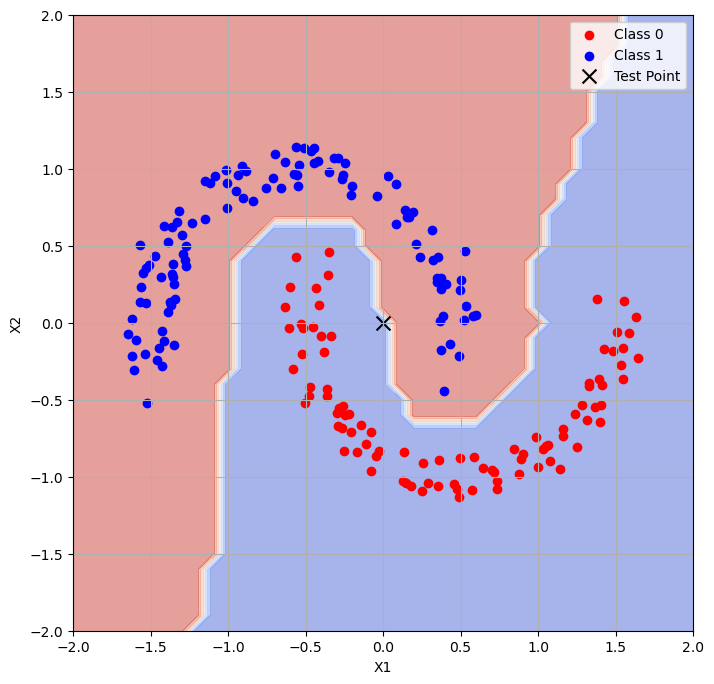
\includegraphics[width=5cm]{D2z.png}
	\end{figure}
	
	\paragraph{Spam filter} Now, we will use 'emails.csv' as our dataset. The description is as follows.
	
	\begin{itemize}
		\item Task: spam detection
		\item The number of rows: 5000
		\item The number of features: 3000 (Word frequency in each email)
		\item The label (y) column name: `Predictor'
		\item For a single training/test set split, use Email 1-4000 as the training set, Email 4001-5000 as the test set.
		\item For 5-fold cross validation, split dataset in the following way.
		\begin{itemize}
			\item Fold 1, test set: Email 1-1000, training set: the rest (Email 1001-5000)
			\item Fold 2, test set: Email 1000-2000, training set: the rest
			\item Fold 3, test set: Email 2000-3000, training set: the rest
			\item Fold 4, test set: Email 3000-4000, training set: the rest
			\item Fold 5, test set: Email 4000-5000, training set: the rest			
		\end{itemize}
	\end{itemize}
	
	\item (8 pts) Implement 1NN, Run 5-fold cross validation. Report accuracy, precision, and recall in each fold.
	
	\begin{soln}  The performance metrics across the 5 folds are as follows:

		\begin{table}[h]
			\centering
			\begin{tabular}{cccc}
				\toprule
				Fold & Accuracy & Precision & Recall \\
				\midrule
				1 & 0.8250 & 0.6545 & 0.8175 \\
				2 & 0.8530 & 0.6857 & 0.8664 \\
				3 & 0.8620 & 0.7212 & 0.8380 \\
				4 & 0.8510 & 0.7164 & 0.8163 \\
				5 & 0.7750 & 0.6057 & 0.7582 \\
				\bottomrule
			\end{tabular}
			\caption{Performance Metrics for 5-Fold Cross Validation}
			\label{tab:results}
		\end{table}
	\end{soln}
	
	\item (12 pts) Implement logistic regression (from scratch). Use gradient descent (refer to question 6 from part 1) to find the optimal parameters. You may need to tune your learning rate to find a good optimum. Run 5-fold cross validation. Report accuracy, precision, and recall in each fold.
	
	\begin{soln}  \[
		\begin{array}{ccccc}
		\toprule
		\text{Fold} & \text{Alpha} & \text{Accuracy} & \text{Precision} & \text{Recall} \\
		\midrule
		1 & 0.001 & 0.918 & 0.8859 & 0.8175 \\
		2 & 0.001 & 0.930 & 0.9027 & 0.8375 \\
		3 & 0.001 & 0.930 & 0.9315 & 0.8134 \\
		4 & 0.001 & 0.954 & 0.9366 & 0.9048 \\
		5 & 0.001 & 0.941 & 0.8997 & 0.9085 \\
		\bottomrule
		\end{array}
		\]
	\end{soln}
	
	\item (10 pts) Run 5-fold cross validation with kNN varying k (k=1, 3, 5, 7, 10). Plot the average accuracy versus k, and list the average accuracy of each case. \\
	
	\begin{soln}  	
	\begin{figure}[h]
		\centering
		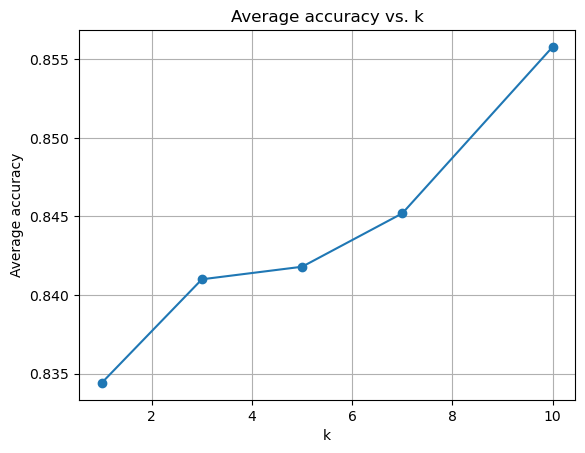
\includegraphics[width=8cm]{Accuracy vs K.png}
	\end{figure} \end{soln}
	
	\item (10 pts) Use a single training/test setting. Train kNN (k=5) and logistic regression on the training set, and draw ROC curves based on the test set. \\
	
	\begin{soln}  
		\begin{figure}[h]
		\centering
		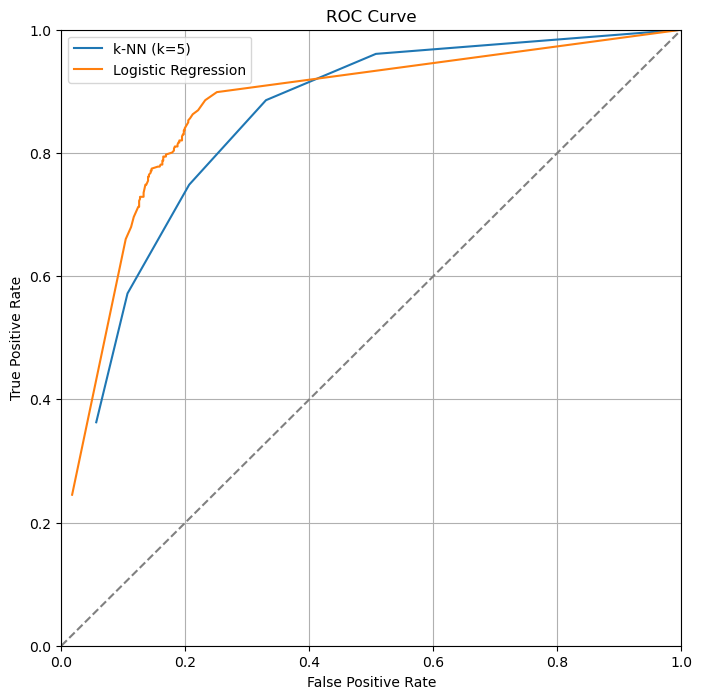
\includegraphics[width=8cm]{ROC KNN Log.png}
	\end{figure} \end{soln}
	
	\end{soln}
	
\end{enumerate}
\bibliographystyle{apalike}
\end{document}
